\section{Dataset i fine-tune amb dades reals}
En aquest projecte no es va obtenir accés a les dades reals fins al mes de gener de 2024. Aquesta data és un any després de l'inici del projecte. Durant aquest any va canviar tant els requisits d'\textbf{i2CAT}, els mètodes de desenvolupament i del sistema plantejats, els coneixements adquirits, els objectius del projecte i, fins i tot, la mentalitat dels desenvolupadors. És aquesta diferència temporal que fa que es vegi com un projecte diferent o l'inici del projecte amb l'arribada de les dades. A més a més, el temps, el maquinari i l'accés el software van ser tan limitants que va haver de centrar-se a trobar una solució per al projecte el més ràpid possible.

\subsection{Descripció general}
Les dades reals consisteixen en una llista de 804 tiquets (700 originalment pactats + 104 de reserva) que van ser seleccionats manualment per \textbf{i2CAT}. D'aquests hi ha aproximadament la meitat d'incidents de \textit{Phishing} o \textit{Spam} i l'altra meitat de \textit{Malware}.

Aquestes dades són significativament més complexes que el \textit{dataset} sintètic utilitzat anteriorment. Les dades d'entrada reals són més llargues i el seu significat és més complicat d'entendre per què és una conversació entre diverses persones per correu. Les entitats que s'ha de trobar també són més llargues, complicades i amb barreres entre categories més difuses del que s'esperava.

\begin{table}[H]
    \centering
    \begin{tabular}{lccr}
        \Xhline{2\arrayrulewidth}
        \textbf{Cua} & \textbf{Recompte} \\
        \hline
        Gestió Incidents (Malware) & 363 \\
        Protecció Perimetre (Phishing / Spam) & 441  \\
        \hline
        \textbf{Total} & \textbf{804} \\
        \Xhline{2\arrayrulewidth}
    \end{tabular}
    \caption{Recompte del nombre de tiquets per cua de la primera selecció de tiquets.}
    \label{tab:recompte_per_cua}
\end{table}

Després d'etiquetar 25 tiquets es va veure que ja majoria de les respostes eren \pyth{"NotFound"}. Això és una mala notícia perquè llavors el model aprendrà que per obtenir molt bon rendiment haurà de contestar sempre el mateix. Mirant més detingudament, es va descobrir que la majoria dels tiquets on succeeix aquest problema són els tiquets de \textit{Malware}, ja que les entitats de sortida no estan fetes per tenir en comptes aquest tipus de tiquets.

Com a resposta, es va plantejar quina seria la millor solució per arreglar aquest problema. Es va plantejar afegir nous camps o crear un model diferent per cada cua. Per culpa de la manca de temps per poder executar cap de les dues solucions, \textbf{i2CAT} va seleccionar 461 tiquets dels 804 previs. D'aquesta nova selecció la majoria són de la cua de Protecció Perímetre tot i que hi ha alguns de Gestió Incidents. També es va escollir aleatòriament 80 tiquets i es van etiquetar. Més tard, aquests tiquets van ser revisats i es va tornar a entrenar els models que havien estat entrenats amb aquestes dades.

\begin{table}[H]
  \centering
  \begin{tabular}{lccr}
      \Xhline{2\arrayrulewidth}
      \textbf{Cua} & \textbf{Recompte} \\
      \hline
      Gestió Incidents (Malware) & 59 \\
      Protecció Perimetre (Phishing / Spam) & 402  \\
      \hline
      \textbf{Total} & \textbf{461} \\
      \Xhline{2\arrayrulewidth}
  \end{tabular}
  \caption{Recompte del nombre de tiquets per cua de la segona selecció de tiquets.}
  \label{tab:recompte_per_cua_2}
\end{table}





\subsection{Exploració de les dades}
Per comprovar la mida de les dades amb les quals es treballa, es creen histogrames i diagrames de caixa.

\subsubsection{Anàlisi de la llarga dels tiquets}
Aquesta anàlisi proporciona informació sobre l'estructura i la complexitat típiques de les dades textuals. Comprendre la distribució de les longituds dels tiquets ajuda a dissenyar els models per manejar eficaçment les diferents longituds d'entrada. A més a més, els valors atípics poden distorsionar les anàlisis i introduir biaixos als models. En eliminar els valors atípics o aplicar les transformacions adequades, els investigadors poden garantir la solidesa i la fiabilitat de les seves anàlisis.

El \textit{boxplot} (diagrama de caixa) de la figura \ref{fig:boxplot_num_chars_tiquets} mostra la distribució del nombre de caràcters dels tiquets, amb una distribució esbiaixada i una caixa de l'amplitud interquartílica desproporcionadament petita a causa de la presència de \textit{outliers} amb recomptes de caràcters excepcionalment alts.

En contrast, el \textit{boxplot} de la figura \ref{fig:boxplot_num_chars_tiquets_outliers} presenta una representació més clara de la distribució de la longitud dels tiquets del conjunt de dades després d'eliminar tots els tiquets amb un recompte de caràcters superior a 10000. L'eliminació d'aquests \textit{outliers} permet veure que la majoria dels tiquets té més de 2000 caràcters i amb molts per sobre dels 5000.

\begin{figure}[H]
    \centering
    \begin{subfigure}{.5\textwidth}
      \centering
      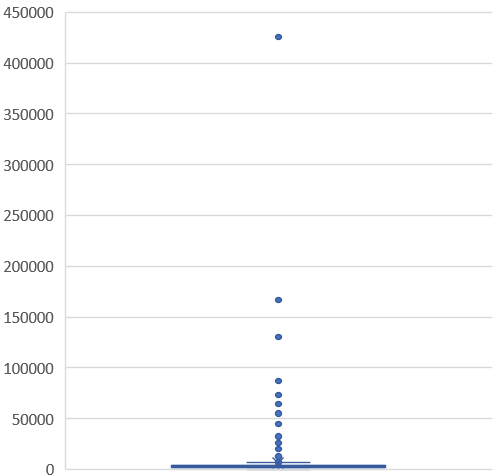
\includegraphics[width=.7\linewidth]{boxplot_num_chars_tiquets.png}
      \caption{Amb totes les sentències.}
      \label{fig:boxplot_num_chars_tiquets}
    \end{subfigure}%
    \begin{subfigure}{.5\textwidth}
      \centering
      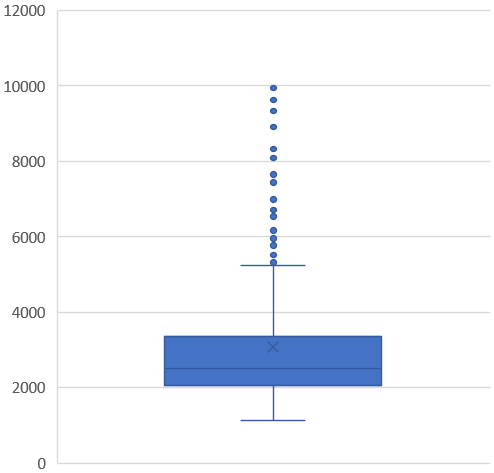
\includegraphics[width=.7\linewidth]{boxplot_num_chars_tiquets_outliers.png}
      \caption{Sense \textit{outliers}.}
      \label{fig:boxplot_num_chars_tiquets_outliers}
    \end{subfigure}
    \caption[Boxplot dels caràcters del text principal de cada tiquet]{Boxplot del nombre de caràcters de cada tiquet. Els tiquets només contenen el text principal. \\ (Creació pròpia)}
    \label{fig:boxplot_num_chars_tiquets_dos}
\end{figure}

A més a més, a les figures \ref{fig:histograma_num_chars_tiquets} i \ref{fig:histograma_num_chars_tiquets_outliers} es pot veure de manera més precisa el recompte de les llargades del nombre de caràcters dels tiquets.

\begin{figure}[H]
    \centering
    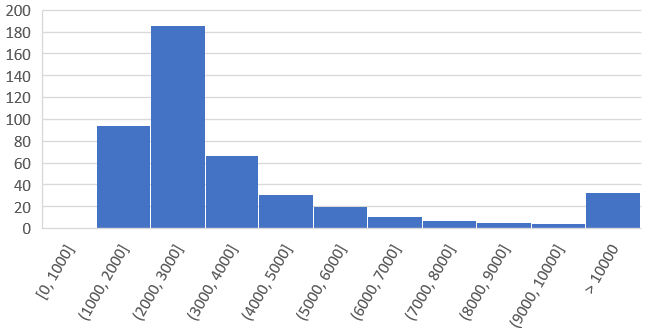
\includegraphics[width=0.9\textwidth]{histograma_num_chars_tiquets.png}
    \caption[Histograma dels caràcters del text principal de cada tiquet]{Histograma del nombre de caràcters de cada tiquet. Els tiquets només contenen el text principal. \\ (Creació pròpia)}
    \label{fig:histograma_num_chars_tiquets}
\end{figure}


\begin{figure}[H]
    \centering
    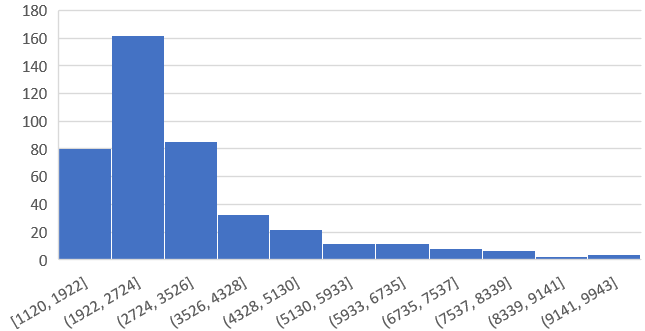
\includegraphics[width=0.9\textwidth]{histograma_num_chars_tiquets_outliers.png}
    \caption[Histograma dels caràcters del text principal de cada tiquet sense outliers]{Histograma del nombre de caràcters de cada tiquet. Els tiquets només contenen el text principal i no s'inclouen els tiquets outliers. \\ (Creació pròpia)}
    \label{fig:histograma_num_chars_tiquets_outliers}
\end{figure}

\subsubsection{Anàlisi de la llargada dels tiquets amb adjunts i referències}
Una petició freqüent va ser afegir més context a cada tiquet, ja que un incident pot estar inclòs en diversos tiquets o pot contenir la resposta d'alguns camps als arxius adjunts. El problema és que amb el maquinari tan limitat, fins i tot entrenar amb només el text principal del tiquet ja és un problema.

A pesar de la limitació d'espai, es va comprovar l'estat de les dades amb aquest context afegit. A les figures \ref{fig:boxplot_num_chars_adj_refs} i \ref{fig:boxplot_num_chars_adj_refs_outliers} es pot veure un \textit{boxplot} de la llargada dels tiquets, amb tots els tiquets i eliminant els 80 \textit{outliers} de més de 10000 caràcters, respectivament. Es pot comprovar que hi ha significativament més caràcters de mitjana respecte a només tenir el text principal, la qual cosa implicaria més temps d'inferència i, en conseqüència, més temps d'entrenament.

\begin{figure}[H]
    \centering
    \begin{subfigure}{.5\textwidth}
      \centering
      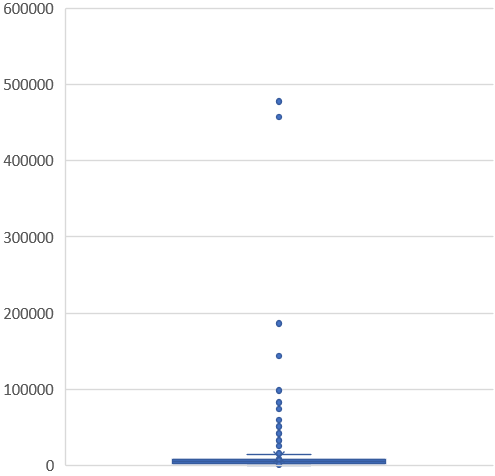
\includegraphics[width=.7\linewidth]{boxplot_num_chars_adj_refs.png}
      \caption{Amb totes les sentències.}
      \label{fig:boxplot_num_chars_adj_refs}
    \end{subfigure}%
    \begin{subfigure}{.5\textwidth}
      \centering
      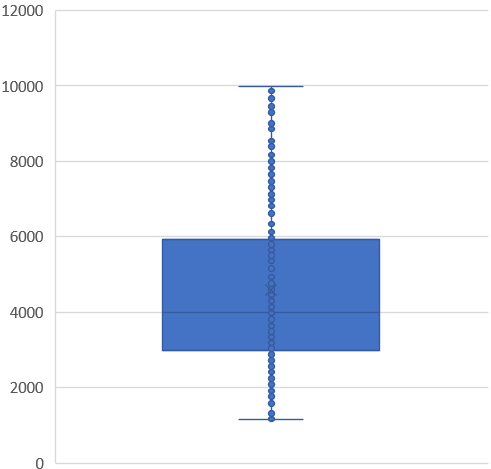
\includegraphics[width=.7\linewidth]{boxplot_num_chars_adj_refs_outliers.png}
      \caption{Sense \textit{outliers}.}
      \label{fig:boxplot_num_chars_adj_refs_outliers}
    \end{subfigure}
    \caption[Boxplot dels caràcters de cada tiquet amb adjunts i referències]{Boxplot del nombre de caràcters de cada tiquet. Els tiquets contenen el text princpial així com el contingut dels fitxers adjunts i les referències a altres tiquets. \\ (Creació pròpia)}
    \label{fig:boxplot_num_chars_adj_refs_dos}
\end{figure}

A les següents figures \ref{fig:histograma_num_chars_adj_refs} i \ref{fig:histograma_num_chars_adj_refs_outliers} es pot veure també la mateixa informació en format histograma.

\begin{figure}[H]
    \centering
    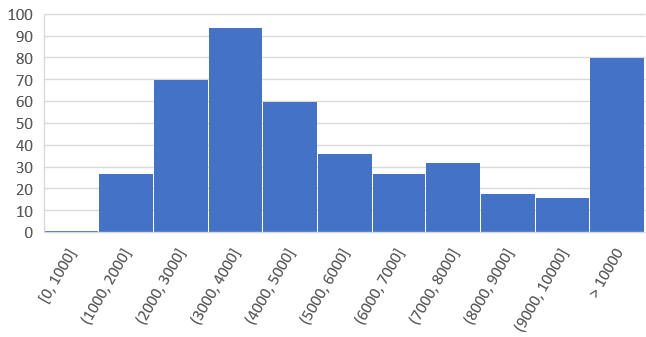
\includegraphics[width=0.9\textwidth]{histograma_num_chars_adj_refs.png}
    \caption[Histograma dels caràcters de cada tiquet amb adjunts i referències]{Histograma del nombre de caràcters de cada tiquet. Els tiquets contenen el text princpial així com el contingut dels fitxers adjunts i les referències a altres tiquets. \\ (Creació pròpia)}
    \label{fig:histograma_num_chars_adj_refs}
\end{figure}

 
\begin{figure}[H]
    \centering
    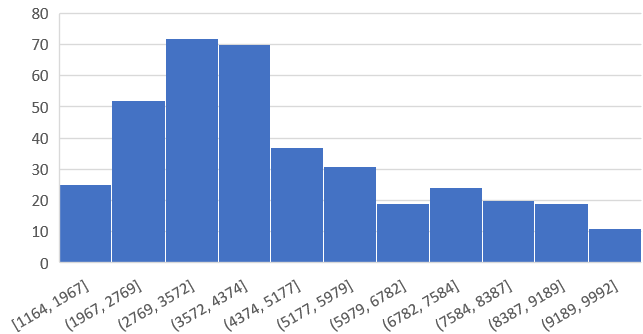
\includegraphics[width=0.9\textwidth]{histograma_num_chars_adj_refs_outliers.png}
    \caption[Histograma dels caràcters de cada tiquet amb adjunts i referències i sense outliers]{Histograma del nombre de caràcters de cada tiquet. Els tiquets contenen el text princpial així com el contingut dels fitxers adjunts i les referències a altres tiquets. També s'ha eliminat els outliers. \\ (Creació pròpia)}
    \label{fig:histograma_num_chars_adj_refs_outliers}
\end{figure}


\subsubsection{Comparació nombre d'adjunts i referències}
En aquesta secció es presenten dos histogrames que il·lustren la distribució dels fitxers adjunts per tiquet i el nombre de referències a altres tiquets.

L'histograma de la figura \ref{fig:histograma_num_adj} indica que la majoria dels tiquets contenen entre 1 i 2 fitxers adjunts, amb alguns valors atípics que contenen més. En segon lloc, l'histograma de la figura \ref{fig:histograma_num_refs} mostra que la gran majoria dels tiquets no contenen referències a cap altre correu. 

\begin{figure}[H]
    \centering
    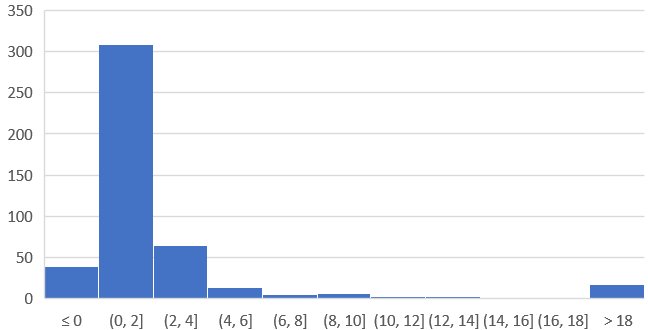
\includegraphics[width=0.9\textwidth]{histograma_num_adj.png}
    \caption[Histograma del nombre d'adjunts a cada tiquet]{Histograma del nombre de arxius adjunts a cada tiquet. \\ (Creació pròpia)}
    \label{fig:histograma_num_adj}
\end{figure}


\begin{figure}[H]
    \centering
    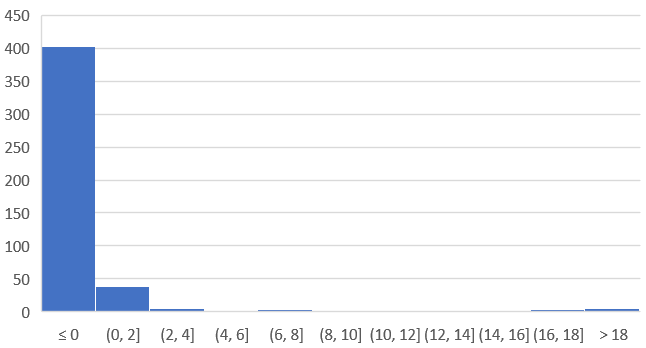
\includegraphics[width=0.9\textwidth]{histograma_num_refs.png}
    \caption[Histograma del nombre de referències a cada tiquet]{Histograma del nombre de referències a altres tiquets a cada tiquet. \\ (Creació pròpia)}
    \label{fig:histograma_num_refs}
\end{figure}

Donats els limitats recursos de maquinari, ha sigut imperatiu optimitzar el procés d'extracció de la informació. En excloure els fitxers adjunts i els tiquets referenciats, s'ha reduït la longitud de la seqüència d'entrada, cosa que es tradueix en temps de processament més ràpid i un menor consum de memòria. Aquesta decisió ha permès obtenir resultats més fiables de l'extracció dels camps sense comprometre el sistema.

\subsubsection{Comparació conjunt de dades d'entrenament i test}
Quan s'analitza un \textit{dataset}, és fonamental assegurar-se que es manté la integritat de les dades en tot moment. En aquest cas, és molt indesitjable que hi hagi un alt percentatge d'entrades sense resposta o, en aquest cas \pyth{"NotFound"}, com s'observa tant al conjunt de dades d'entrenament com al de prova.

La presència d'un nombre significatiu d'entrades \pyth{"NotFound"} introdueix un biaix a l'anàlisi. Això distorsiona les mètriques, la qual cosa porta a percepcions i conclusions inexactes. En conseqüència, els models entrenats amb aquests \textit{datasets} poden tenir dificultats per generalitzar bé dades no vistes. L'absència d'informació a la partició d'entrenament impedeix la capacitat del model per extrapolar coneixements a instàncies noves amb precisió.

A continuació es pot veure a les taules \ref{tab:stats_dataset_1} i \ref{tab:stats_dataset_2} el percentatge dels camps de sortida que no es poden contestar amb la informació proporcionada al tiquet. Es pot observar també que els percentatges de camps no trobats gairebé no canvia entre versions, però com s'ha pogut veure, ha tingut unes implicacions més grans a l'hora de l'entrenament.

S'ha de notar que si es tingués en compte el contingut dels arxius adjunts i dels tiquets que es referencien, aquests percentatges disminuirien lleugerament, però encara serien majoritàriament \pyth{"NotFound"}.

{\setlength{\tabcolsep}{1pt}   %Espai a la dreta i esquerra de cada cel·la amb text
\begin{table}[H]
    \centering
    \begin{tabular}{lcccccccc}
        \toprule
        Mètrica 
        & \begin{tabular}{@{}c@{}}affected \\ Users\end{tabular}
        & \begin{tabular}{@{}c@{}}mitigation \\ Actions\end{tabular}
        & \begin{tabular}{@{}c@{}}control \\ Actions\end{tabular}
        & \begin{tabular}{@{}c@{}}urlMail \\ Incident\end{tabular}
        & \begin{tabular}{@{}c@{}}fromMail \\ Incident\end{tabular}
        & \begin{tabular}{@{}c@{}}recipientMail \\ Incident\end{tabular}
        & \begin{tabular}{@{}c@{}}subjectMail \\ Incident\end{tabular} 
        & Total \\         
        \midrule
        \makecell[l]{ NotFound \\ \textit{test} } & 80.0\% & 73.3\% & 93.3\% & 86.6\% & 60.0\% & 66.6\% & 73.3\% & 76.1\% \\ 
        \makecell[l]{ NotFound \\ \textit{train} } & 70.0\% & 56.2\% & 100.0\% & 91.2\% & 41.2\% & 56.2\% & 58.7\% & 67.6\% \\
        \bottomrule
    \end{tabular}
    \caption[Estadístiques de la primera versió del \textit{dataset}]{Estadístiques de la primera versió del \textit{dataset} amb el percentatge de camps no trobats (\textit{NotFound}).}
    \label{tab:stats_dataset_1}
\end{table}
}

{\setlength{\tabcolsep}{1pt}   %Espai a la dreta i esquerra de cada cel·la amb text
\begin{table}[H]
    \centering
    \begin{tabular}{lcccccccc}
        \toprule
        Mètrica 
        & \begin{tabular}{@{}c@{}}affected \\ Users\end{tabular}
        & \begin{tabular}{@{}c@{}}mitigation \\ Actions\end{tabular}
        & \begin{tabular}{@{}c@{}}control \\ Actions\end{tabular}
        & \begin{tabular}{@{}c@{}}urlMail \\ Incident\end{tabular}
        & \begin{tabular}{@{}c@{}}fromMail \\ Incident\end{tabular}
        & \begin{tabular}{@{}c@{}}recipientMail \\ Incident\end{tabular}
        & \begin{tabular}{@{}c@{}}subjectMail \\ Incident\end{tabular} 
        & Total \\         
        \midrule
        \makecell[l]{ NotFound \\ \textit{test} } & 60.0\% & 73.3\% & 93.3\% & 86.6\% & 60.0\% & 60.0\% & 73.3\% & 72.3\% \\ 
        \makecell[l]{ NotFound \\ \textit{train} } & 50.0\% & 63.7\% & 97.5\% & 92.5\% & 56.2\% & 52.5\% & 61.2\% & 67.6\% \\ 
        \bottomrule
    \end{tabular}
    \caption[Estadístiques del \textit{dataset} corregit]{Estadístiques de la segona versió del \textit{dataset} amb les correccions amb el percentatge de camps no trobats (\textit{NotFound}).}
    \label{tab:stats_dataset_2}
\end{table}
}
